\documentclass[12pt,info]{asg}
% General info for the asg.cls file to load
\usepackage[normalem]{ulem}
\Instructor{Anna Koop}
\Campus{University of Alberta, Augustana}
\Email{akoop@ualberta.ca}
\Office{Heather Brae 1-31}
\Class{AUCSC 370}
\ClassTitle{Programming Languages}
\Term{Fall 2016}
\Department{Department of Science}


\AsgNum{Final.2}
\AsgTitle{Assigning Preferences}
\Due{11:55pm, Dec 14, 2016}
\Total{30}

\title{Assigning Ranked Preferences}

\begin{document}

\maketitle
\section*{Objectives}
\begin{itemize}
\item To demonstrate your ability to think in different programming styles.
\item To examine the strengths and weaknesses of Scheme, Prolog, and C in a real-world problem.
\item To experience and reflect on how different programming paradigms approach the same problem.
\end{itemize}

\section*{Problem Specification}
Beginning in 2017, First-year students to Augustana will be enrolled in a "First Year Seminar", a 3-week discussion-based research course designed to introduce new students to university-level scholarship. A wide variety of seminars have been proposed, but space is limited.

New students will be asked to pick their top  choices from the available classes. Then comes the difficult task of actually assigning students to classes in a way that respects physical constraints (no more than 25 per class, and only one offering of each class) while optimizing happiness (as much as possible we want people to get their top choices).

For next year, students will be choosing through a online form that outputs an Excel-compatible file. Someone will be manually processing that file in order to assign students to classes in as fair and accommodating a way as possible. Of course this raises a lot of questions about what is fair and how student preferences should be taken into account. And for all of those questions, how strong is the effect of the answer? 
%Are three choices from every student enough, considering we want to minimize random assignment as much as possible? Will students tend to select only a small number of classes or will we have a good variety of interest? What is a reasonable minimize size of class? How many classes do we need to provide as options?

\section*{Program Specification}
Computers (somewhat) to the rescue. You will write three versions of the program for doing this course assignment: one in C, one in Scheme, and one in Prolog. We will use a simple scoring mechanism for evaluating the quality of the match. The match will give every student a disappointment number: 0 if they got into their first choice, 1 for second, 2 for third, and 5 for being assigned one they did not choose. The total score is the sum over all students. 

This means 0 is perfection---everyone got into their first choice. Highly unlikely. Optimizing the assignment is a difficult problem in general so you {\em do not} have to find the single best solution for the given data. The score is simply to evaluate the quality of your program's solution.

\subsection*{Input}

The data structures and control flow are completely up to you and, of course, will be different for each language.
\sout{The input you have to work with will be in two text files. First gives the full list of course identifiers and possible associated information, eg:}
You may hard-code classes into your source rather than deal with file input and output. Class identifiers are formatted as FYSXXX where XXX is a unique number for each class, eg:
\begin{lstlisting}[language=Lisp]
	FYS111, Drugs
	FYS112, Murder!
	FYS113, How to be a Doctor
	FYS114, Machine Apocalypse
	...
\end{lstlisting}

The most significant data structure gives a list of students and their top three preferences. Student numbers again may be made up however you like as long as each student has a unique numeric identifier.
\begin{lstlisting}[language=Lisp]
	1011111, FYS114, FYS111, FYS122
	1011112, FYS111, FYS122, FYS199
	...
\end{lstlisting}

A third thing you may consider (but do not have to implement) is how other student information may be factored in: for example, time of registration, per-class diversity of student body in personal background and majors, etc. Discussing how these might be considered and how they would affect the assignment algorithm will be an excellent way to demonstrate critical thought.

\subsection*{Output}
Your program will read these files and display a table assigning students to each class:
\begin{lstlisting}[language=Lisp]
	FYS111, 1011111, 1011113, 1011114, 1022222...
	FYS112, 1111112, 1011112, 1011115, 1022223...
	...
\end{lstlisting}

A proper solution must satisfy the following characteristics:
\begin{itemize}
\item All students are assigned to one and only one class.
\item All student identifiers are valid.
\item All class identifiers are valid.
\item No class has more than \sout{25} X or less than \sout{10} Y students.
\item No class has less than \sout{10} Y students
\item \sout{The matching score passes a minimum bar}\footnote{\sout{TBD and posted in eClass}
Given we do not have access to a full-sized data file, I will be manually evaluating quality according to the metric given with your test structures.
}.
\end{itemize}

You should set up your code such that the maximum and minimum number of students can be easily adjusted. Since we are manually entering the data for now, you will not be expected to include the 300 or so students that will actually be using the system. Rather, your code should be set up such that it is easy to adjust the input and numbers appropriate.

\section*{Report}

In addition to the three program files, you will submit a (no more than 3-page) report. Your report should examine the strengths and weaknesses of each particular language {\em and} overall language paradigm for the task. 

\subsection*{Introduction}
Start with a brief, high-level description of your approach in each language. This includes what data structures and control flow you used or took into account.

\subsection*{Body}
The focus of the report is on comparing and contrasting your use of the languages for this problem. What was different about the algorithm or program structure in each? What was similar? You may include personal details (eg. difficulty, time) as well as technical information (eg. efficiency, readability, etc).

A secondary aspect of the report is providing critical observations of the algorithms used. Independent of the code itself, what did you find in the quality of the solutions? What things does the programmer of the ultimate assignment code need to consider? What Excel macros (i.e. short functions) will be useful/critical to simplify the process for them?

\subsection*{Conclusion}
Conclude with a recommendation for the 'best' language for this problem. Be sure to support your recommendation appropriately.

This is a formal report and you will be graded on clarity, structure, and grammar as well as the critical thought and  knowledge demonstrated in the report.


\section*{Grading}

Each program is marked out of 50 and worth 5\% of your final grade. The report is marked out of 60 and is worth 15\% of your final grade.

\subsection*{Program Code}
Code compiles (on park) according to instructions and/or runs in the (web-based) interpreters without error. /15

The results are displayed in a readable format according to the specification. The results are valid according to the given criteria. /10

The code is well documented and readable. /10

The solution approach is appropriate for the given language. /10

The code demonstrates skill in the language constructs and idioms. /5

\subsection*{Report}
The report is complete. It provides overview, detail, and comparison between all the languages as described in the specification. /10

The report is well organized, grammatically correct, and clear. /10

The report is factually correct and accurately explains relevant concepts. /20

The report demonstrates thoughtfulness and insight in relation to both project and course concepts. /20


%%%%%%%%%%%%
%\begin{figure}[bt]
%\label{fig:adder}
%\centering
%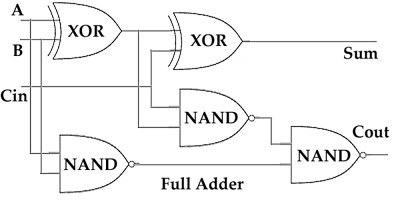
\includegraphics[width=.6\textwidth]{full_adder.png}
%\caption{A (claimed) full-adder circuit}
%\end{figure}

%\newcounter{rubricCat}
%\newcounter{rubricVal}
%\newlength{\colwidth}

%\newenvironment{rubric}[1]{%
%	\setcounter{GradeCategories}{#1}
%	\begin{landscape}
%	\begin{table}[t]
%	\begin{center}
%	\begin{tabulary}{.8\textwidth}{ l | *{5}{c}}
%	 & Excellent & Good & Acceptable & Needs Work & Absentee \\
%	 \end{tabulary}
%	 \end{center}
%	 \end{table}
%	\end{landscape}
%} % rubric environment

\end{document}
